\documentclass[conference]{IEEEtran}
\usepackage{graphicx}
\usepackage{todonotes}
\usepackage{listings}
\usepackage{textcomp}
\usepackage{url}
\usepackage{biblatex}
\addbibresource{references.bib}

\begin{document}
\title{Replication of Zhang et al. 2017 \cite{ZhangsMainPaper}}
\author{\IEEEauthorblockN{Oliver Goldstein}
\IEEEauthorblockA{og14775@my.bristol.ac.uk}
\and
\IEEEauthorblockN{Robert Stamper}
\IEEEauthorblockA{rs13197@my.bristol.ac.uk} }

\maketitle

\IEEEpeerreviewmaketitle

\section{Introduction}

Reliable image classification has been a problem in the computer vision community since its inception. Recently the introduction of self driving cars has motivated the need for  reliable, accurate and fast classifications. Traffic sign recognition has been an important research area for driving assistance, traffic-sign maintenance, and unmanned vehicles \linebreak

In 1996, a state of the art implementation \cite{Old2003Paper} achieves accuracy levels of no more than 94\%, with processing times of up to 15 - 20 seconds, using Hough transforms, FEX and Kalman filters. Recently, the field has changed massively with artificial neural networks (ANN's) displaying near perfect discriminative performance dealing with computer vision classification tasks, even after adjusting for class distributions. \linebreak

In the following paper, we attempt to replicate the results of \cite{ZhangsMainPaper} which claimed to achieve 99.87\% accuracy classifying street signs using only a shallow network architecture. In our implementation, we achieved 89.9\% accuracy at first attempt and after improvements (IX), achieved 98.76\%.

\section{Related Work}

\cite{ZhangsMainPaper} details a history of Traffic Sign Recognition (TSR). In this section, three papers with competitive accuracy levels shall be detailed, with a short elaboration on the drawbacks and advantages of each approach. The following 3 papers are sampled from 2011 onwards to give context to how the approaches and accuracies have changed over the last six years. \linebreak

TSR consists of 3 steps; 1) data pre-processing, 2) feature extraction and 3) classification of the input images. 
\subsection{Data Processing}

Data processing in \cite{Paper1} occurs with normalization in 3 similar ways to the way we have implemented our normalization step. All of the methods, \cite{Paper1}\cite{Paper2}\cite{Paper3} use data augmentation of some kind, for example random translations and random rotations.

\subsection{Feature Selection} 

With respect to feature selection, \cite{Paper1}\cite{Paper2} \& \cite{Paper3} all use some combination of HOG and HAAR features, which have been used for a long time in computer vision applications. \cite{Paper1} uses these with MLPs (Multi Layer Perceptrons) trained on these features. \cite{Paper2} uses HOG features. It then uses two sliding windows, one which is small or coarse and one which is large or fine. The coarse sliding window establishes ROIs and uses NMS to suppress multiple nearby ROIs, with the small window ensuring detection and the large window size ensuring high recall and precision. A Hough transform is then applied to detect red equilateral triangles, to ensure a higher accuracy on mandatory and danger images. Due to perspective alignment representing a challenge for the Hough transform, eight class specific SVMs (one for each of the images) are trained on the regions to determine which sign is in the image. \cite{Paper3} uses a HOG descriptor with both signed and unsigned gradient orientations, which are fed into an ELM learning algorithm which is a simplified feedforward neural network, with one hidden layer for efficiency.

\subsection{Classification} 

When making a final classification \cite{Paper1} establishes a committee, which is used with an average of the posterior class probabilities to finalise a classification. The paper does not mention its classification time per frame. \cite{Paper1} in 2011 achieves an error rate only 0.6\% behind that of [2], whilst with a remarkably similar architecture to \cite{Paper1}. In addition \cite{Paper1} has an efficient GPU implementation and it builds directly on from LeCun 1998. However, LeCun 1998 does not use a max pooling layer, instead using a subsampling layer. The max pooling layer gives significant positional invariance over larger local regions.

\begin{figure}[ht]
    \centering
    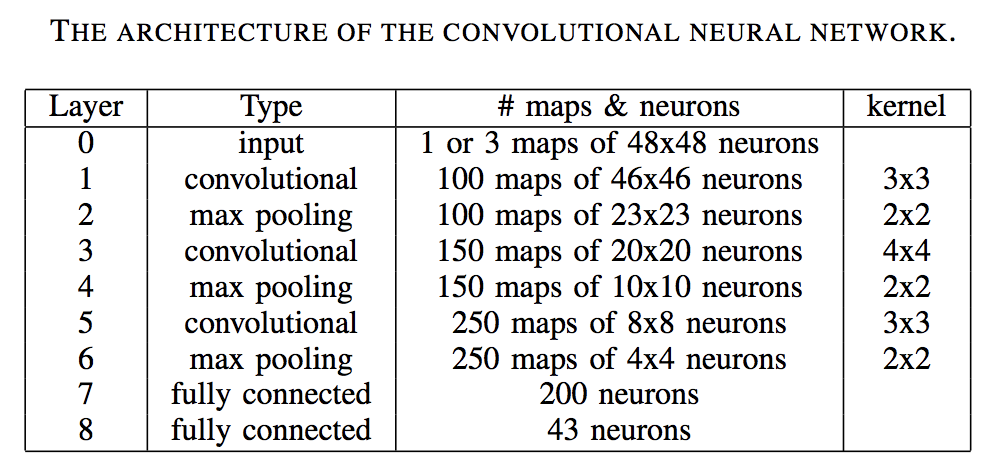
\includegraphics[width=0.45\textwidth]{network_structure.png}
    \caption{The structure of \cite{Paper1}.}
    \label{fig:network_structure}
\end{figure}

\begin{figure}[ht]
    \centering
    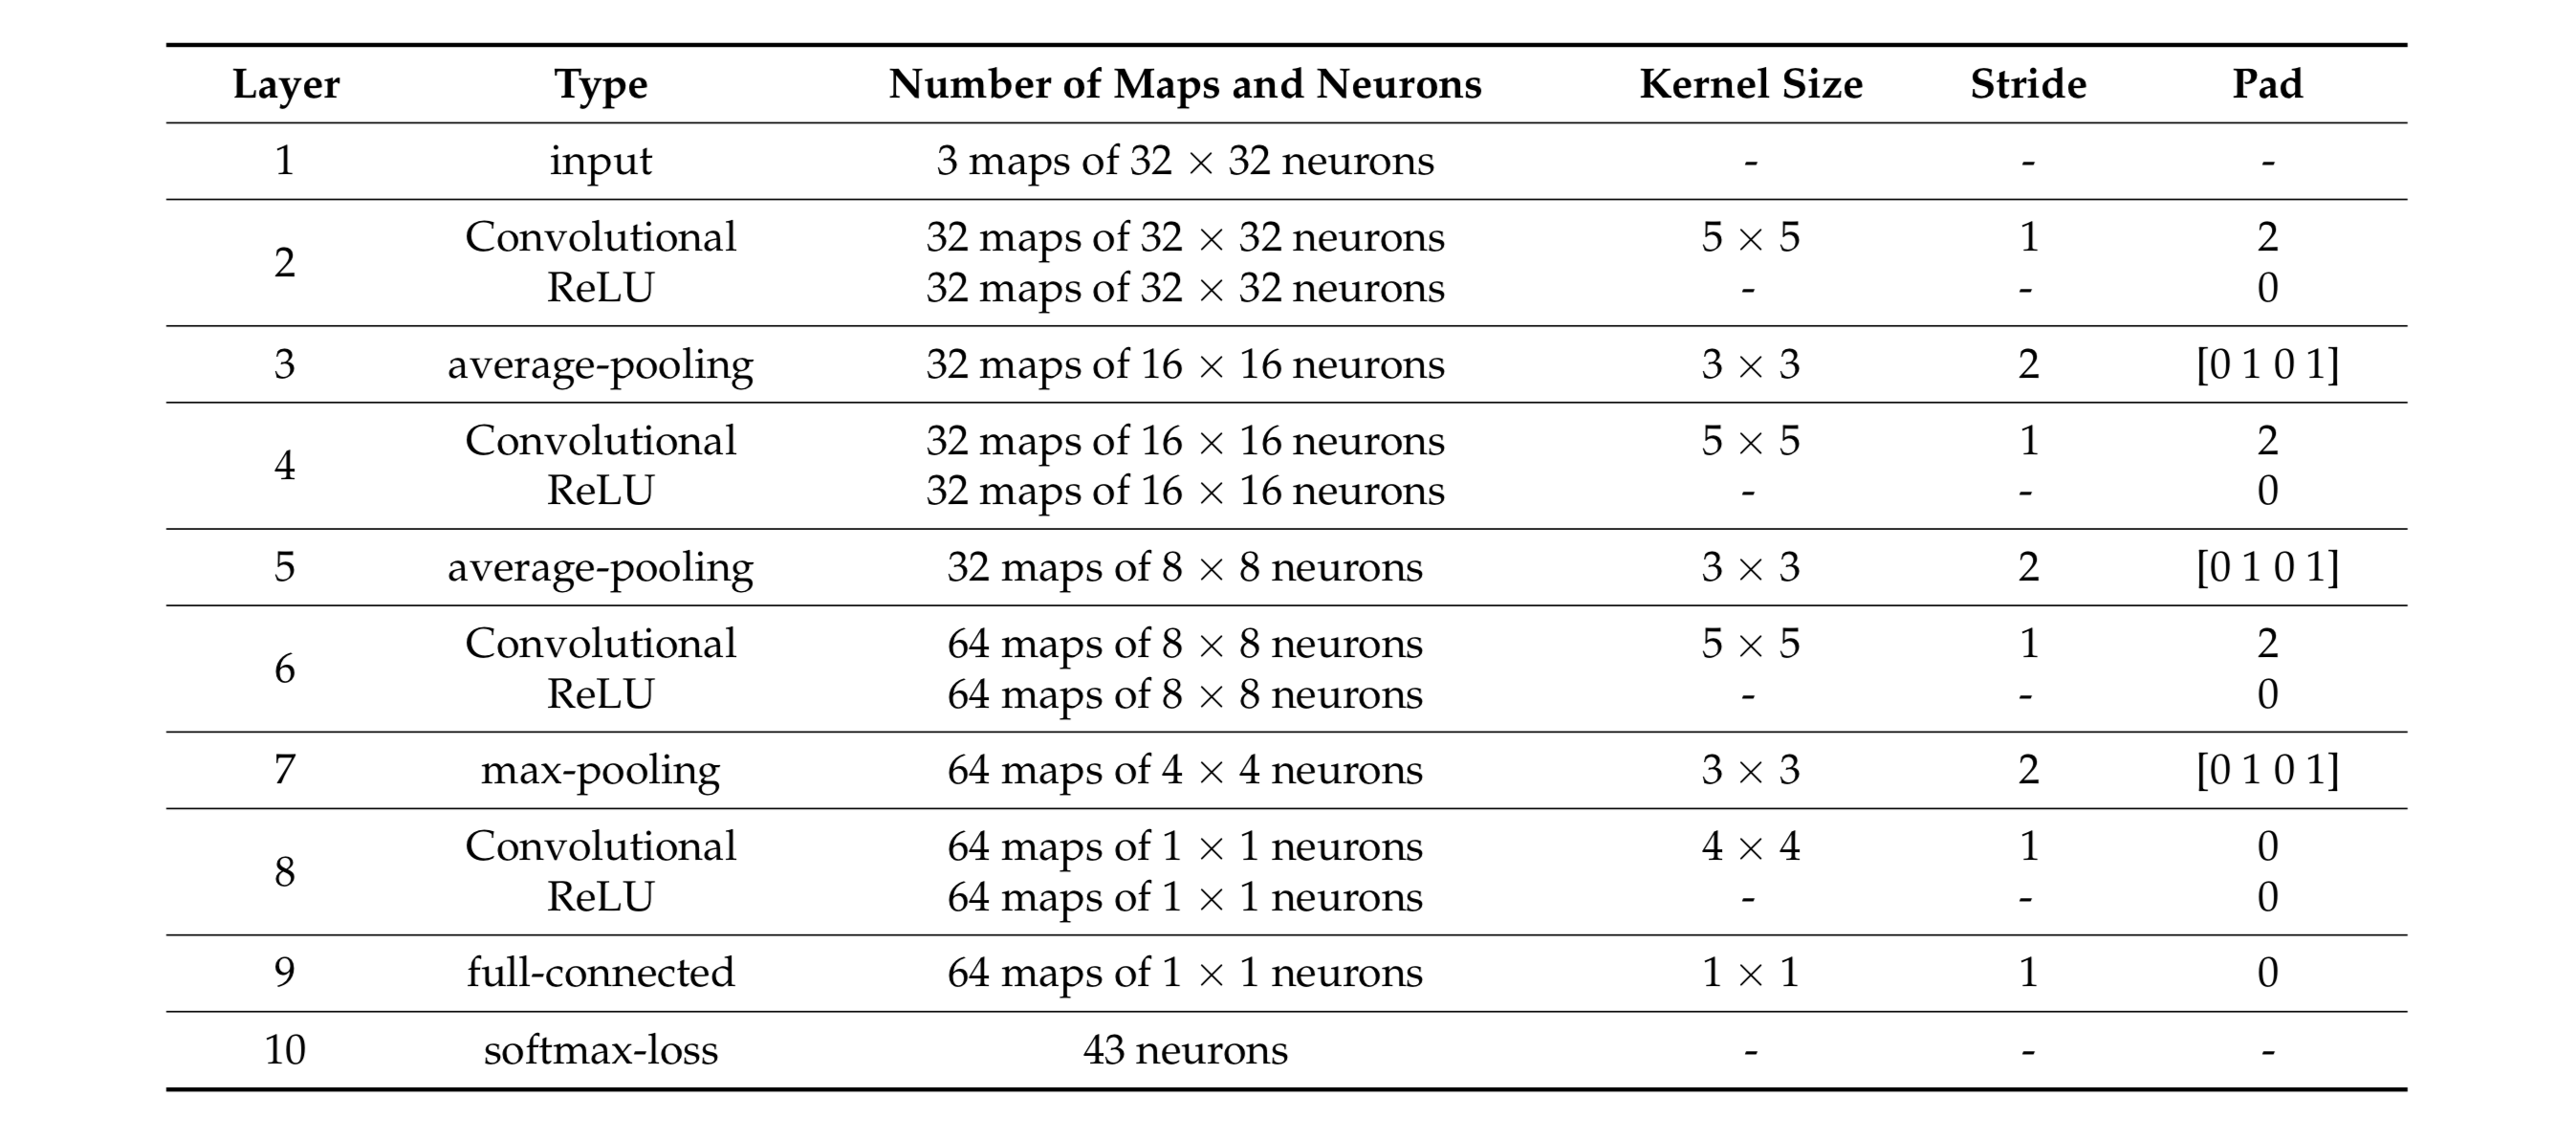
\includegraphics[width=0.45\textwidth]{zhang_network_structure.png}
    \caption{The structure of \cite{ZhangsMainPaper}.}
    \label{fig:zhang_structure}
\end{figure}

\cite{Paper2} uses a combination of SVMs and Hough transforms. It takes over a second to classify. \cite{Paper3} simply uses the constructed SFNN and takes 1.4ms/frame to classify. \cite{Paper1} 2011 claims an accuracy of 99.15\%, \cite{Paper2} in 2013 claims an accuracy of 99.85\% plus and \cite{Paper3} in 2016 claims an accuracy of 99.54, 100, 98.33, 99.94, 98.96 and 99.95 for speed limits, other, de-restriction, mandatory, danger and unique - respectively.

\section{Dataset}

\begin{figure}[ht]
    \centering
    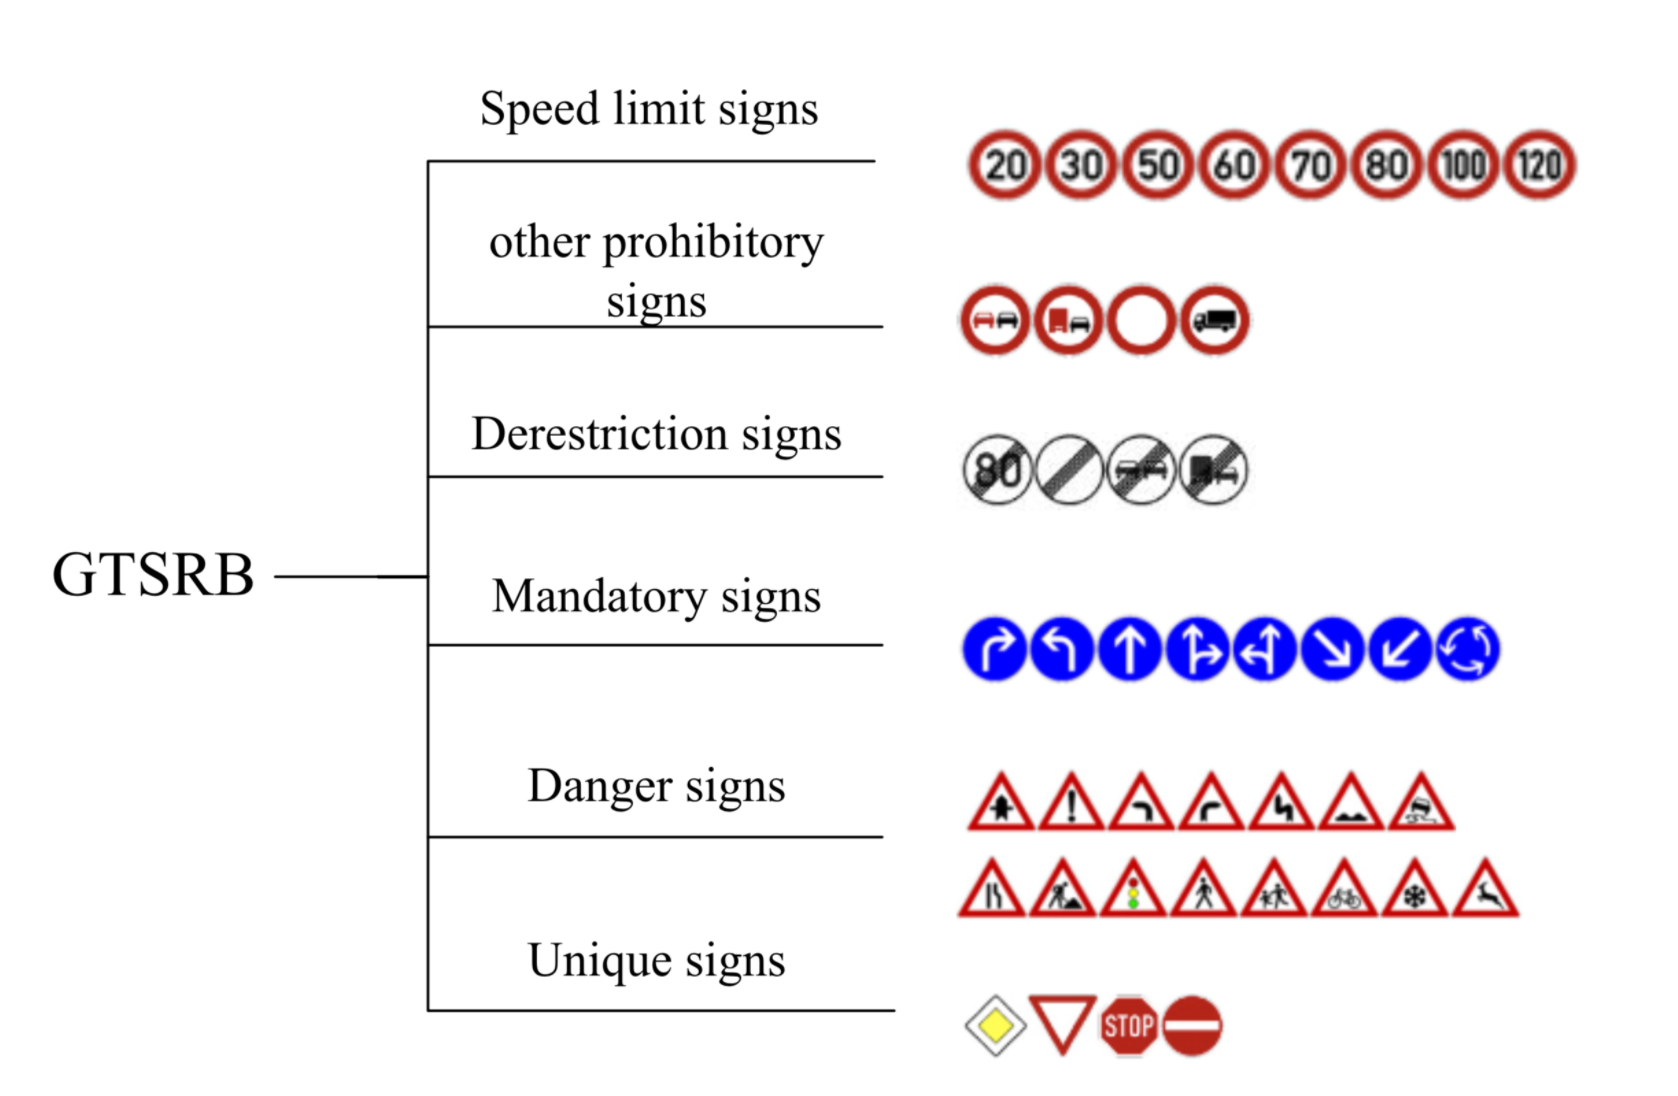
\includegraphics[width=0.45\textwidth]{traffic_signs.png}
    \caption{The image types contained within the GTSRB dataset.}
    \label{fig:zhang_structure}
\end{figure}

The dataset was GTSRB, which uses single-image, multi-class classification problems with close to 50 classes and more than 50,000 lifelike images in total, contained in a database. The dataset consists of 39,209 training images, 12,630 test images. The class labels were encoded by a one hot vector which are contained in the dataset. The data was contained in a .pkl file which is a serialized python object where the fields are accessed in the same way as a Python array. More specifically, when parsed, it is a list of two tuples, where each tuple is an array of images and an array of labels.

\section{Method (Zhang et al)}

The 10 layer inception architecture implemented by \cite{ZhangsMainPaper} is divided into two distinct sections. The first 7 layers are a mixture of convolution, ReLu and sub-sampling layers (inc. the input layer). The use of average-average-max layer ordering was determined by trying all $2^{3}$ combinations of max or average types. The remaining layers are fully connected layers, finally driven through soft-max loss. The network is trained with SGD, on a set of weights initialized from a uniform distribution, with the same update rule that was used in AlexNet. Pre-processing of the images occurs, in particular image whitening, where the covariance of each image is manipulated to be the identity matrix. The authors seem to use a variety of ad hoc explanations for various parameter values, for instance they fix the stride value to be 2 to prevent the speed of sub-sampling from being too fast, or the addition of methods such as whitening only after empirical testing. However, the guiding theme throughout the paper is that they focus on producing a shallow network, which has the added bonus of having a recognition time of 0.64ms/frame on a single CPU.

\section{Implementation Details}

The implementation of the paper was done on an Nvidia P100 GPU \cite{TeslaP100}. The most challenging step in the implementation was to implement the AlexNet update rule which was not in the core TensorFlow framework. The majority of the inception architecture was trivially implemented with standard TensorFlow methods in namespaces such as tf.layers. 

The TensorFlow Momentum Optimizer splits up the minimize method into two separate steps, when modifying the gradient wrt. an objective function. In particular, compute\_gradients and apply\_gradients, which I shall refer to as CG and AG respectively. CG calculates the value of the gradients with respect to the cross entropy loss.

The TensorFlow Momentum Optimizer has the form:
\newline
\newline
\footnotesize
\texttt{accumulation = momentum * accumulation + gradient \newline
variable -= learning rate * accumulation}
\normalsize

\begin{figure}[ht]
    \centering
    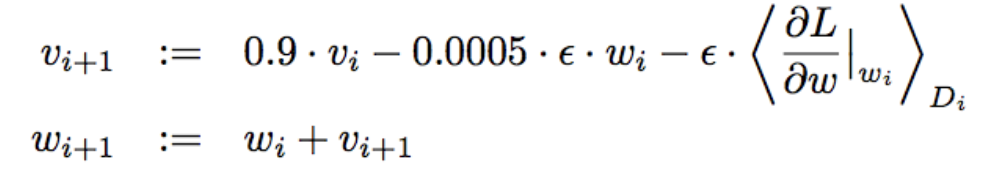
\includegraphics[width=0.45\textwidth]{AlexNet.png}
    \caption{AlexNet update rule}
    \label{fig:alexnet}
\end{figure}

After analysis, we discovered three things; first that each weight has a corresponding momentum variable in the TensorFlow optimizer, mirroring the AlexNet update rule in Figure \ref{fig:alexnet}. This is an important semantic distinction which would have grossly affected results otherwise. Second, the \texttt{gradient} value in the Momentum Optimizer mirrored the ith batch average loss derivative in the AlexNet paper. Third, the weight update rule included an unwanted minus sign in TensorFlow, so by setting the learning rate to -1, instead there would be an addition there which was desired. By hand coding the learning rate in the rule itself, we were able to replicate the wanted learning rate. The following python function \texttt{change\_gradients(grads, weights)} serves to act as the update rule:
\newline
\newline
\texttt{exp1 = tf.multiply(weight\_decay, learning\_rate) \newline
    exp2 = tf.scalar\_mul(exp1, weights) \newline
    exp3 = tf.negative(exp2) \newline
    }
    \newline
    At this point exp3 = weight\_decay * learning\_rate * w\_i
    \newline
    The remainder of the code constructs exp6 = learning\_rate * loss
    \newline
    \newline
\texttt{
    exp4 = tf.scalar\_mul(learning\_rate, grads) \newline
    exp5 = tf.negative(exp4) \newline
    exp6 = tf.add(exp5, exp3) \newline
    return exp6 \newline
}

At this point, the updated weights were applied using AG. With the update rule implemented and the overall architecture as close as possible to the paper, we performed a substitution which was due to the similarity of negative log loss and cross entropy loss, whereby we substituted cross entropy loss for negative log loss due to the faster implementation in TensorFlow.

Initially, we decided to map data pre-processing functions over the data set whilst training, but after realizing that this was pre-processing every image in the whole dataset once every few hundred training rounds, we replaced the entire data set. The final training time was 10 minutes. Because of technical issues with BlueCrystal, we could not record the recognition time per frame.

\section{Replicating Figures}

\begin{figure}[ht]
    \centering
    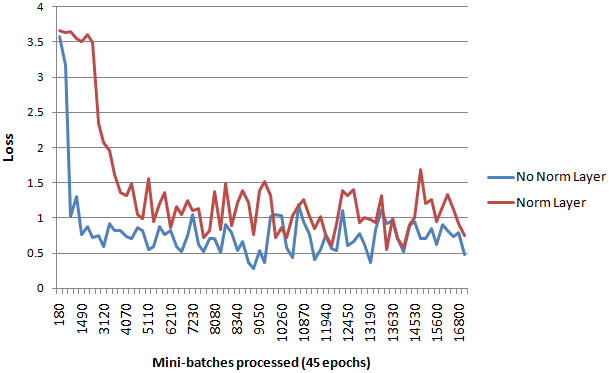
\includegraphics[width=0.5\textwidth]{Figure3a.png}
    \caption{Training Loss with normalisation layer and without}
    \label{fig:normloss1}
\end{figure}
\begin{figure}[ht]
    \centering
    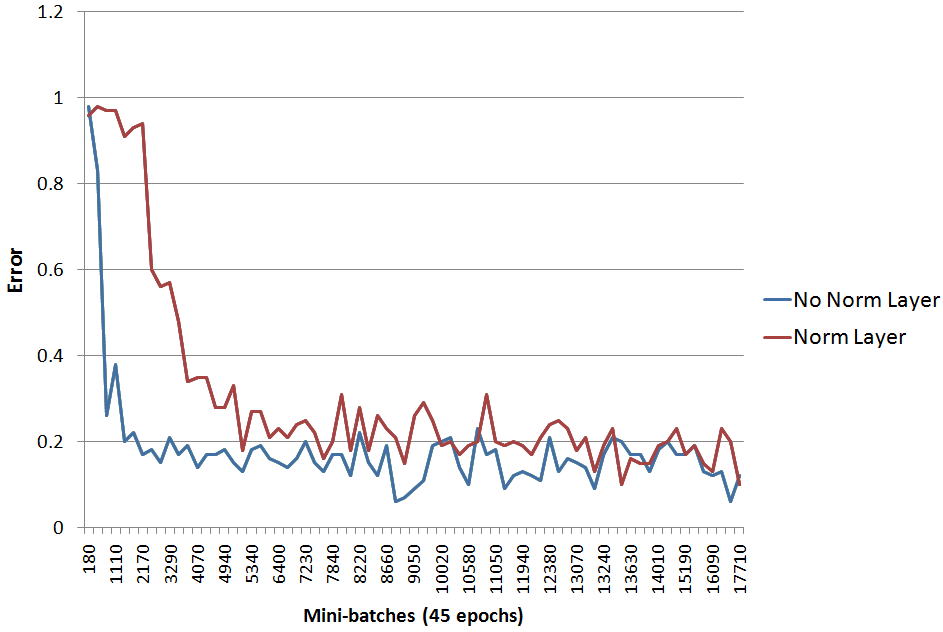
\includegraphics[width=0.5\textwidth]{Figure3b.png}
    \caption{Validation error with normalisation layer and without}
    \label{fig:normloss2}
\end{figure}
\begin{figure}[ht]
    \centering
    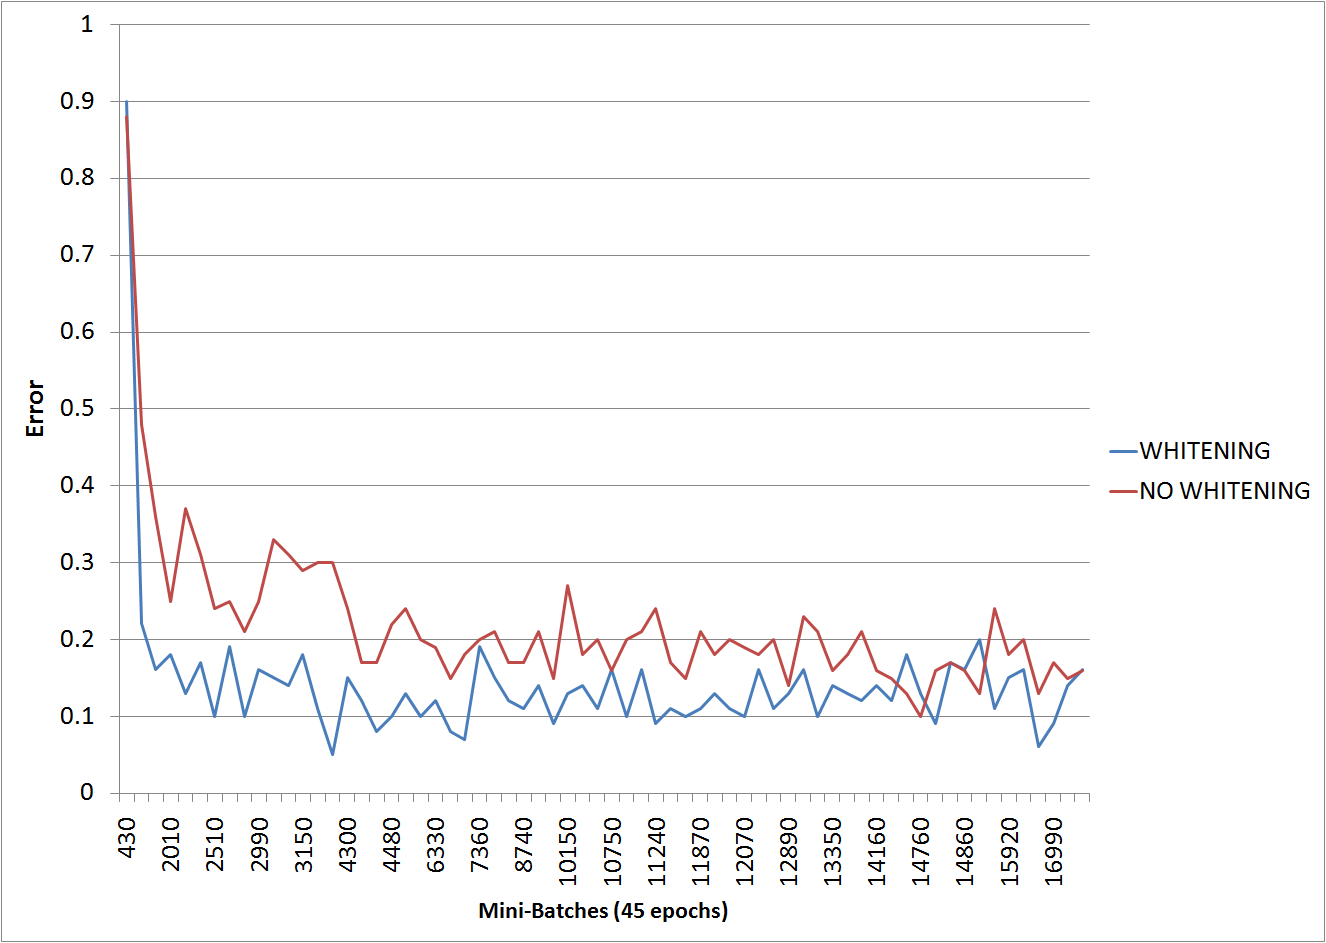
\includegraphics[width=0.5\textwidth]{Figure4.png}
    \caption{Training with whitening cs training without whitening}
    \label{fig:whitening}
\end{figure}
\begin{figure}[ht]
    \centering
    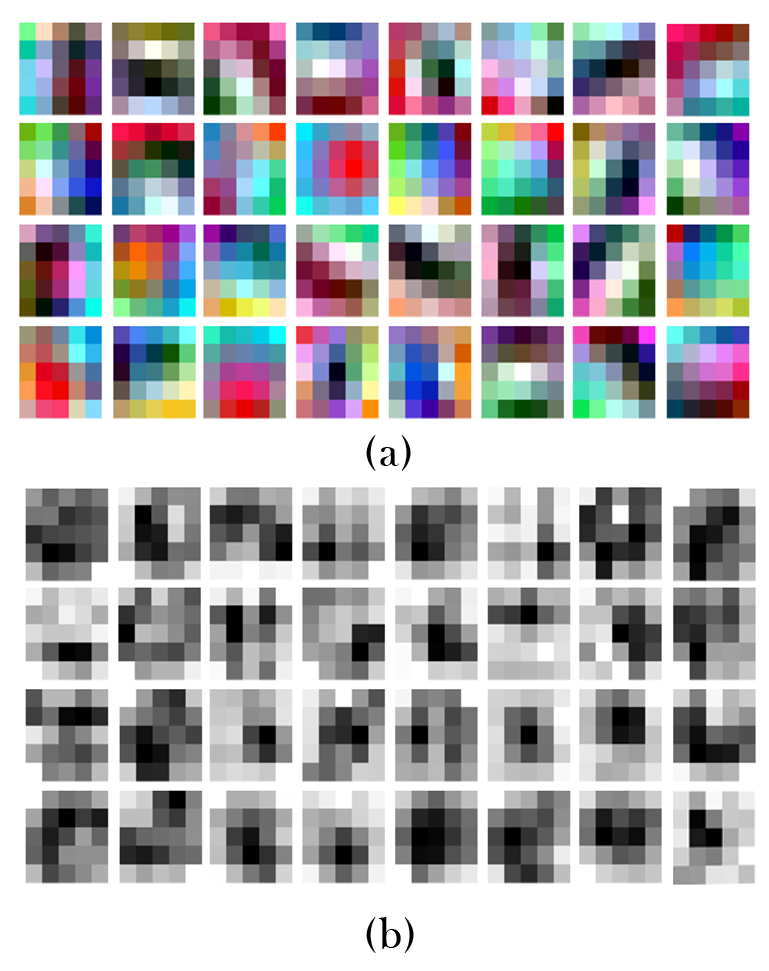
\includegraphics[width=0.5\textwidth]{conv_filters.png}
    \caption{Convolution filters from the first and second layer}
    \label{fig:filters}
\end{figure}

\section{Replicating quantitative results}
\begin{center}
\begin{tabular}{ |c|c|c| }
 \hline
 Zhang et al & 99.84 \\ 
 Ensemble CNN's & 99.65 \\
 Committee of CNNs & 99.6 \\ 
 CNN+ELM & 99.40 \\
 Human(best individual) & 98.84 \\
 Our Improved Method & 98.76 \\
 Complementary Features & 98.65 \\
 Multi-Scale CNN & 98.31 \\
 SHOG5-SBRP2 & 98.17 \\
 HOS-LDA & 97.84 \\
 Our Method & 89.56 \\
 
 \hline
\end{tabular}
\end{center}
\begin{table*}[t]
\caption{Individual results for subsets of traffic signs}
\centering
\begin{tabular}{p{0.12\linewidth}p{0.12\linewidth}p{0.12\linewidth}p{0.12\linewidth}p{0.12\linewidth}p{0.12\linewidth}p{0.12\linewidth}}
\hline
Method & Speed Limits & Other Prohibitions & Derestrictions & Mandatory & Danger & Unique \\
\hline
HOGv+KELM & 99.54 & 100 & 98.33 & 99.94 & 98.96 & 99.95 \\
\hline
Complementary Features & 98.56 & 99.73 & 92.50 & 99.55 & 97.31 & 99.90 \\
\hline
Multi-Scale CNNs  & 98.61 & 99.87 & 94.44 & 97.18 & 98.03 & 98.63 \\
\hline
Committee of CNNs & 99.47 & 99.93 & 99.72 & 99.89 & 99.07 & 99.22 \\
\hline
Human (Best Individual) & 98.32 & 99.87 & 98.89 & 100 & 99.21 & 100 \\
\hline
Zhang et al & 99.93 & 99.80 & 99.44 & 100 & 99.13 & 99.90 \\
\hline
Our Replication Attempt & 91.02 & 90.70 & 97.14 & 92.94 & 71.47 & 97.25 \\
\hline
Our Attempt + Improvements & 98.31 & 99.07 & 93.81 & 98.81 & 96.52 & 99.61 \\
\end{tabular}
\end{table*}

\section{Discussion}

The final accuracy we achieved was not remotely close to 99.84\% quoted by Zhang et Al. We copied their network as closely as possible, within reasonable bounds when faced with ambiguity, but the highest accuracy we managed to achieve within 45 epochs without additional improvements was 89.56\%. 

We were surprised by the ambiguous language in the paper. For example, we implemented image 'whitening' on an image by image basis. We later found out that they had most likely done it by taking means and standard deviations channel-wise across the whole dataset. We changed our implementation to do this instead, but surprisingly it decreased our accuracy, so we carried on using whitening on a per image basis.

\begin{figure}[ht]
    \centering
    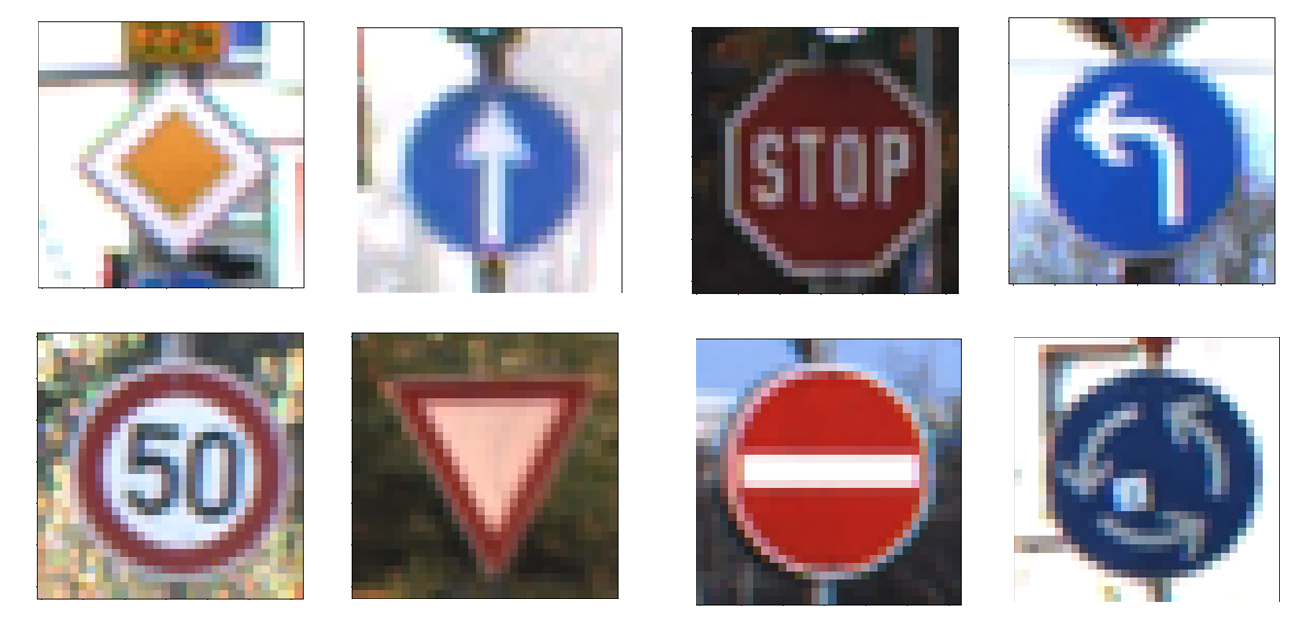
\includegraphics[width=0.5\textwidth]{Successes.png}
    \caption{Successfully classified signs}
    \label{fig:successes}
\end{figure}
\begin{figure}[ht]
    \centering
    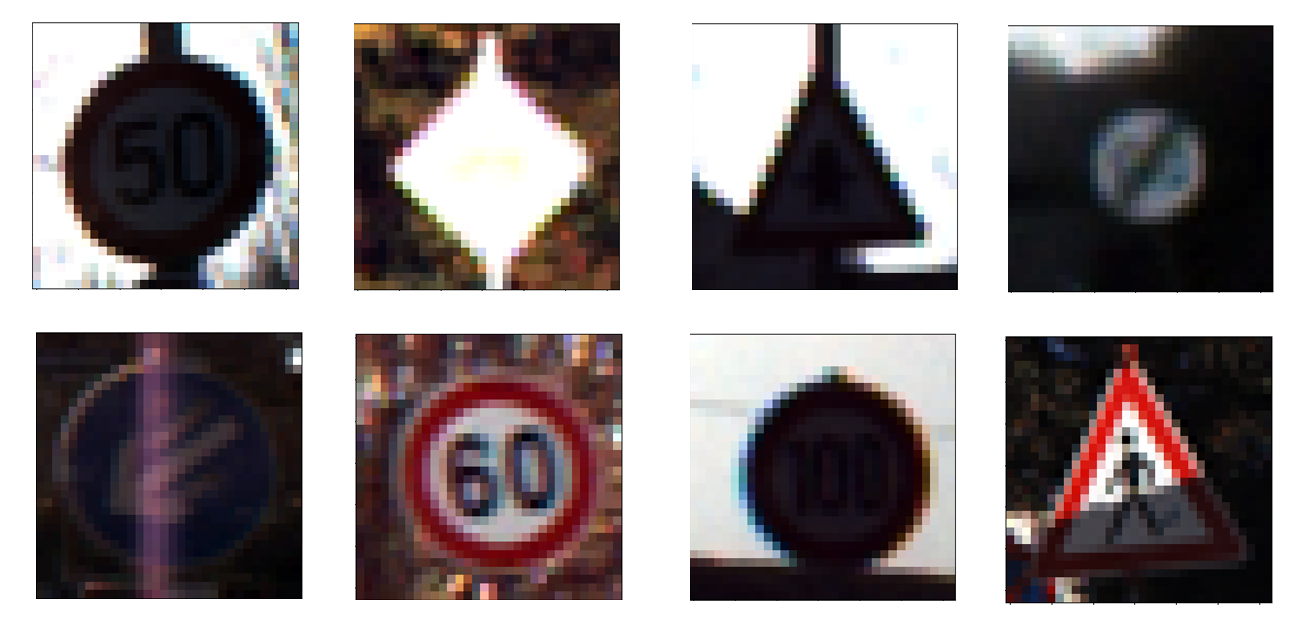
\includegraphics[width=0.5\textwidth]{Failures.png}
    \caption{Some examples of failures}
    \label{fig:failures}
\end{figure}

Figures \ref{fig:failures} \& \ref{fig:successes} show some failure and success cases of the model. The traffic signs the network had the hardest time dealing with were those which were very dark and had extremely high contrast. Whilst we did not examine the individual logit vectors to understand where maximum uncertainty was, manually examining the failure cases, we noticed that the failure cases were generally predictable. The overly dark or overly light images accounted for a large proportion of the failed classifications. The success cases are well lit and reasonably clear. However, even some failures were very clear indicating a deep confusion with the robustness of the network at hand.

The accuracy that the replication achieved whilst conforming to the papers specification loosely was close to 90\%, which is an utterly absurd difference indicating a profound replicability crisis at the heart of artificial neural network research. We suspect the authors used dropout without mentioning it.

\section{Improvements}

\subsection{Neuronal Dropout}

Dropout is commonly implemented in neural networks to reduce overfitting. Overfitting is a danger in networks that have many parameters and small amounts of data. That said, there is some debate over how useful dropout is on convolutional layers, considering they have small numbers of parameters. Srivastava, Hinton et al\cite{Dropout_Paper} explain that droput acts as a regularisation technique acting in a similar way to bagging. For each training example some subset of the units are probabilistically completely disabled. A neural network is now seen as $2^{n}$ thinned neural networks and the authors show that by taking the resulting network with all units enabled is an approximate averaging technique over all of the networks. This method also prevents complex co-adaptations between neuronal units, which the authors establish by making reference to a genetic analogy.

In light of this, we added dropout to all of our convolutional layers and our fully connected layers. We settled on keep probabilities of (0.9, 0.75, 0.75) for the three convolution layers respectively and 0.5 for all fully connected layers.

\subsection{Additional training iterations}

When we were trying to replicate the Zhang et el. paper we tried to follow their method exactly, so we kept the training to 45 epochs as they did. However, now that we were implementing improvements we chose to run the model for 150 epochs, testing the entire test set after each epoch, recording all of the values and then selecting the highest one at the end. Performing this procedure with the original model without additional improvements we reached 91.5\%, up from 89.6\%.

We were expecting a small increase in accuracy but dropout had a dramatic effect on the accuracy of the model. Adding dropout increased the maximum accuracy over 150 epochs by approximately six percent.

\subsection{Contrast Adaptive Histogram Equalization}
As seen before, a lot of the failure classifications consisted of dark, high contrast images. One way of tackling this issue is by using Contrast Adaptive Histogram Equalization. This uses a set of bins which contain contrast information where the size of each bin is determined by an algorithm to optimize for histogram equalization, which refers to the reallocation of contrast within the image. Applying this to the data set improved the accuracy by approximately one percent. Our highest accuracy with improvements was 98.76\%

\begin{figure}[ht]
    \centering
    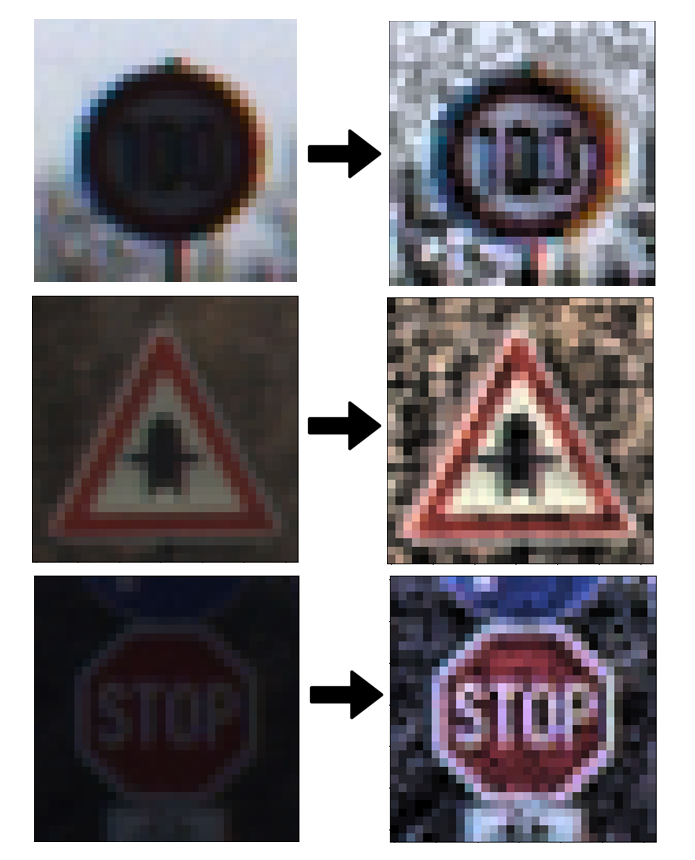
\includegraphics[width=0.5\textwidth]{Histogram_Normalisation.png}
    \caption{Convolution filters from the first and second layer}
    \label{fig:adaptiveHistogram}
\end{figure}

\section{Conclusion and Future Work}

Due to the non-deterministic effects taking place within the network the claims of the authors are practically impossible to falsify and this paper recommends at the very least the provision of code, a cross framework random seed (or list) which can be used to replicate findings involving randomness, the dataset used (if it has been augmented in any way) and the outputted model when providing results. Any paper refusing to do this should not be taken seriously within the research community, especially when the improvements year on year are so marginal. Future work would be taken to identify why even the clearest of images are sometimes classified incorrectly and whether additional assumptions and architectural structure placed within the network can be used to improve classification performance in the future. Focus should be on structural modifications of networks rather than small improvements in accuracy.

\printbibliography
%\bibliographystyle{plain}
%\bibliography{references}

\end{document}
